
Um sinal � um conjunto de dados ou informa��es, que podem descrever diversos tipos de fen�menos, como um sinal de telefonia ou de voz (Figura \ref{fig:Voice}), o registro de vendas de uma empresa ou ainda os valores de fechamento de uma bolsa de valores (Figura \ref{fig:CotacaoBovespa}) \cite[p.~75]{Lathi}. Segundo \citeonline[p.~1]{Oppenheim} existe uma linguagem adequada para descrever sinais e um conjunto poderoso de ferramentas para analis�-los, capaz de se aplicar a problemas oriundos de diversos dom�nios. A s�rie de Fourier e a Transformada R�pida de Fourier s�o ambas exemplos destas ferramentas, e ser�o apresentadas nos pr�ximos cap�tulos.

\vspace{5.0mm}

\begin{figure}[H]
	\centering
	\captionsetup{width=0.8\textwidth, font=footnotesize, textfont=bf}	
	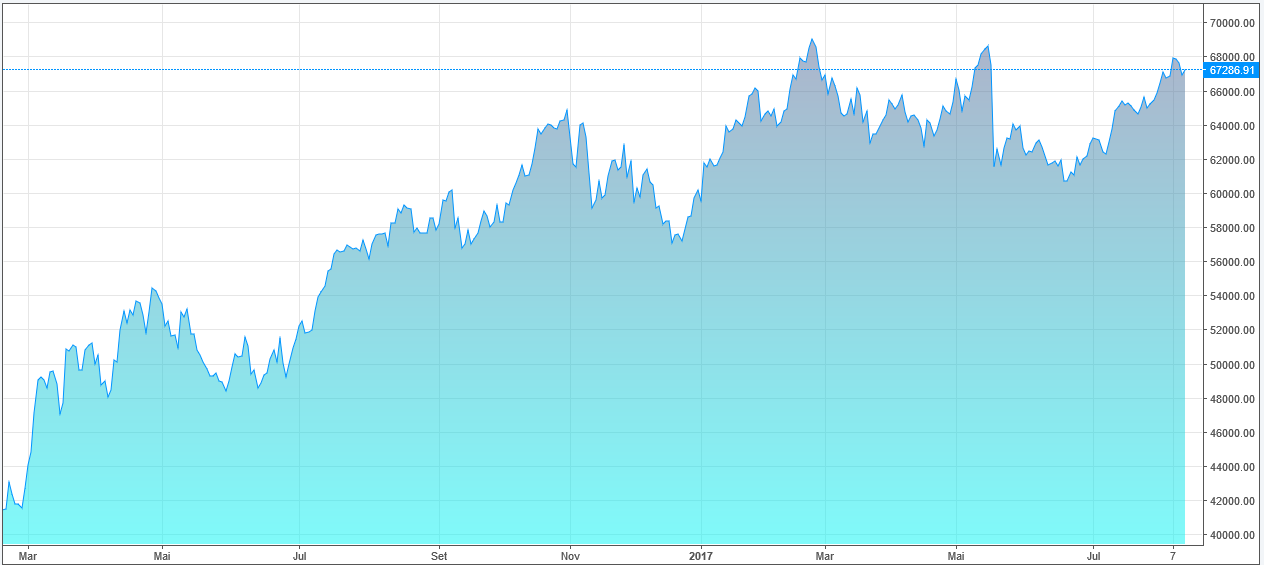
\includegraphics[width=0.8\linewidth]{Images/RevisaoDeLiteratura/CotacaoBovespa.png}
	\caption{�ndice BM \& FBOVESPA, S�o Paulo - Brasil}
	\vspace{-3.5mm}
	\caption*{Fonte: \citeonline{bovespa}}
	\label{fig:CotacaoBovespa}
\end{figure}

\begin{figure}[H]
	\centering
	\captionsetup{width=0.8\textwidth, font=footnotesize, textfont=bf}	
	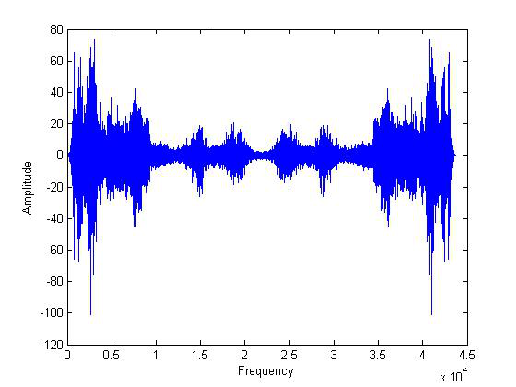
\includegraphics[width=0.8\linewidth]{Images/RevisaoDeLiteratura/Voice.pdf}
	\caption{Sinal Refer�ncia de Voz}
	\vspace{-3.5mm}
	\caption*{Fonte: \citeonline{NirmalRaj}}
	\label{fig:Voice}
\end{figure}


\section{Sistemas de Tempo Continuo e Tempo Discreto}
	%\input{src/RevisaoDeLiteratura/STCTD.tex}

\section{S�rie de Fourier}
	
A s�rie de Fourier tem como principio os estudos das somas trigonom�tricas de senos e cossenos harmonicamente relacionados,  com o intuito de descrever fen�menos peri�dicos. Tal estudo possui uma longa hist�ria que data pelo menos da �poca dos babil�nicos, e que envolve  o estudo de diferentes fen�menos f�sicos. Mas o marco moderno neste tema ocorre em 1748 com o matem�tico e f�sico su��o Leonhard Paul Euler \cite[p.~104]{Oppenheim}. Euler em seu estudo sobre ondas estacion�rias atrav�s de cordas vibrantes observou que se a configura��o da posi��o vertical $y_0$ de um ponto horizontal $x$ em uma onda estacionaria  no tempo $t_0$ for uma combina��o linear dos modos normais da onda, o mesmo acontece com a configura��o em qualquer valor de tempo $t_s$ subsequente. Com base nesse estudo Euler demonstrou que � poss�vel calcular diretamente os coeficientes da combina��o linear em tempos futuros usando os coeficientes em tempos anteriores. \cite[p.~104]{Oppenheim}.  

\vspace{6mm}
\begin{figure}[H]
	\centering
	\captionsetup{width=0.8\textwidth, font=footnotesize, textfont=bf}	
	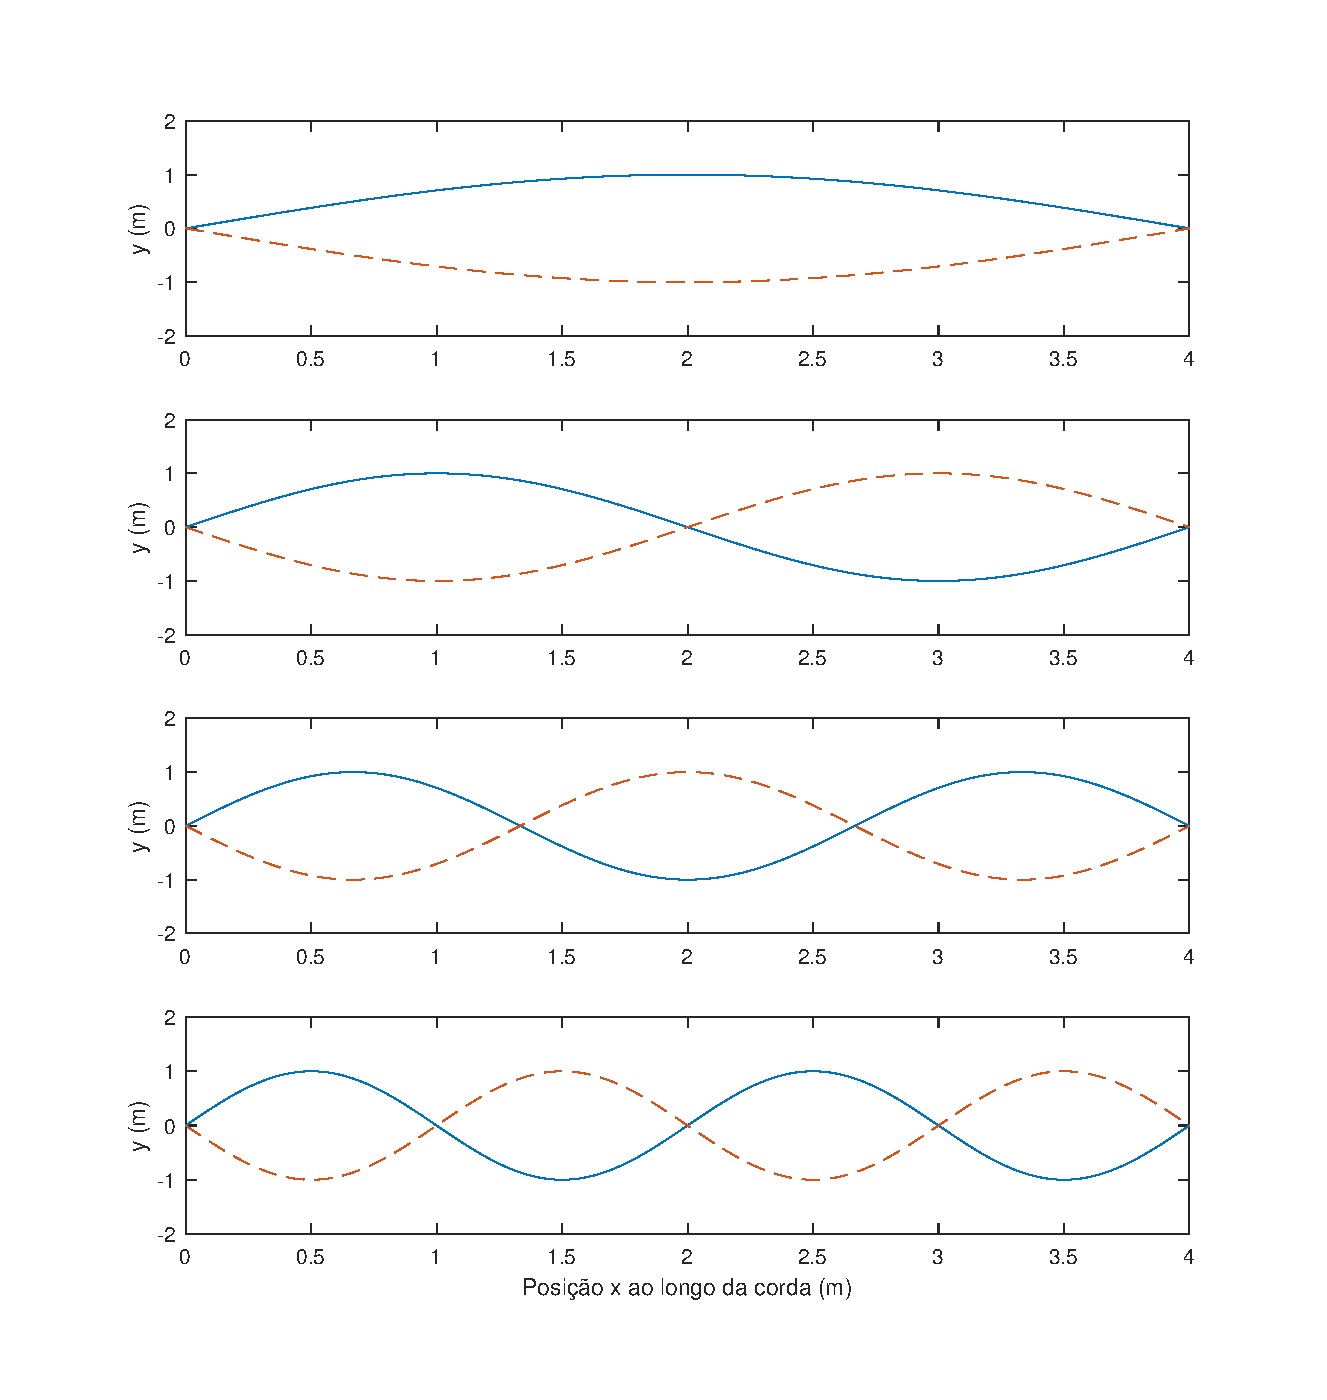
\includegraphics[width=0.8\linewidth]{Images/RevisaoDeLiteratura/OndasEstacionarias.eps}
	\caption{Modos Normais de uma Corda Vibrante}
	\vspace{-3.5mm}
	\caption*{Fonte: Adaptado de \citeonline[p.~105]{Oppenheim}}
	\label{fig:OndasEstacionarias}
\end{figure}
\vspace{6mm}


O estudo de Euler se tornam ainda mais importantes quando aplicado a sinas e a sistemas LIT. Segundo \citeonline[p.~163]{Haykin}, se a entrada de um sistema Linear Invariante no Tempo (LIT) for expressa por uma combina��o linear ponderada de sen�ides ou exponenciais complexas, a sa�da do sistema ser� expressa como uma combina��o linear ponderada da resposta do sistema a cada sen�ide ou exponencial complexa. Expressar sinais em termo de senoides ou exponenciais complexas n�o apenas leva a uma express�o alternativa �til para o comportamento da entrada e sa�da de um sistema LTI, como tamb�m fornece uma caracteriza��o muito criteriosa dos sinais e sistemas. 

Segundo \citeonline[p.~105]{Oppenheim}, meio s�culo depois da divulga��o do trabalho de Euler, o f�sico e matem�tico franc�s Jean-Baptiste Joseph Fourier (1768 - 1830), havia se envolvido no estudo sobre s�ries trigonom�tricas, com a motiva��o f�sica de estudar o fen�meno da propaga��o e difus�o de calor. Fourier conclui que  s�ries senoidais harmonicamente relacionadas eram �teis na representa��o da distribui��o de temperatura em um corpo, e que 'qualquer' sinal peri�dico poderia ser representado po tal s�rie. Fourier ainda apresentou uma representa��o para sinais aperi�dicos, n�o atrav�s de somas ponderadas de senoides harmonicamente relacionadas, mas como integrais ponderadas de senoides que n�o s�o necessariamente harmonicamente relacionadas\cite[p.~163]{Haykin}.

Como afirma \citeonline[p.~106]{Oppenheim}, muitas das ideias b�sica por tr�s das contribui��es de Fourier j� eram conhecidas, e as condi��es precisas sob as quais a representa��o de sinais proposta era v�lida s� foram apresentadas por P.L. Dirichlet em 1829. Por�m foi Fourier que que teve a clara percep��o do potencial pra essa representa��o, e at� certo ponto foi o seu trabalho e suas afirma��es que estimularam grande parte do trabalho subsequente. Logo em sua homenagem o estudo de sinais e sistemas, usando representa��es senoidais, � denominado an�lise de Fourier. E as s�ries pelo qual � realizada a representa��o de sinais na forma de somas de senoides complexas � denominada s�rie de Fourier. 

\subsection{Resposta do Sistemas LTI a Entrada Senoidal} 

Na an�lise de Fourier, os sinais de entrada senoidais s�o comumente usados para caracterizar a resposta de um sistema Linear e Invariante no Tempo, ou LTI (Linear Time-Invariant). A resposta senoidal em estado estacion�rio de um sistema LTI � obtido pela convolu��o entre a entrada senoidal e o sinal de impulso\cite[p.~163]{Haykin}. 

Ao aplicar um sinal impulso ($\delta (t)$) a entrada de um sistema LTI,  � gerado um sinal de sa�da conhecido como resposta ao impulso $\delta (t)$. Atrav�s da resposta ao impulso � poss�vel caracterizar de maneira completa o comportamento de um sistema. A resposta ao impulso tamb�m possibilita conhecer a resposta do sistema LTI a qualquer sinal de entrada, atrav�s da convolu��o deste sinal ao impulso \cite[p.~108]{Haykin}.    

Assim realizando a convolu��o do impulso ao sinal senoidal, segundo \citeonline[p.~164]{Haykin}, a sa�da de um sistema LTI dado uma entrada senoidal complexa $x(t)$, na forma exponencial $e^{j \omega t}$, � dada por:

\begin{equation}
	y(t) = H(j \omega) e^{j \omega t}
	\label{eq:SaidaSenoideComplexa}
\end{equation}

Em que $H(j \omega)$ � a resposta em frequ�ncia, definida em termos de resposta ao impulso $\delta (t)$. Assim;

\begin{equation}
	H(j \omega) = \int_{-\infty}^{\infty} \delta (t) e^{-j \omega t} dt
	\label{eq:RespostaSenoideComplexa}
\end{equation}

Logo a entrada senoidal complexa em um sistema LTI gera uma sa�da igual a entrada senoidal multiplicada apenas pela resposta em frequ�ncia do sistema $H(j \omega)$. 

As equa��es (\ref{eq:SaidaSenoideComplexa}) e (\ref{eq:RespostaSenoideComplexa}) apenas consideram como entrada um sinal senoidal. Por�m � de interesse obter uma express�o para a resposta do sistema LTI a quaisquer sinais arbitr�rios. Para tal \citeonline[p.~164]{Haykin} considera a senoide complexa $\psi~=~e^{j \omega t}$ como uma autofun��o do sistema $H$ associando com o autovalor $\lambda~=~H(j \omega)$, de modo a satisfazer:

\begin{equation}
	H\| \psi \| ~=~ \lambda \psi (t)
\end{equation}

Como pode ser visto na Figura (\ref{fig:PropriedadeDeAutofuncao}), a sa�da de um sistema dada a entrada de uma autofun��o, � o produto da entrada por um n�mero complexo. Se $e_k$ for um autovetor de uma matriz $A$, e $\lambda_k$ os autovalores associados a esta matriz,  a autorrela��o do problema tradicional do autovalor matricial � aplic�vel, $A e_k ~=~ \lambda_k e_k$ \cite[p.~164]{Haykin}.

\vspace{6mm}
\begin{figure}[H]
	\centering
	\captionsetup{width=0.8\textwidth, font=footnotesize, textfont=bf}	
	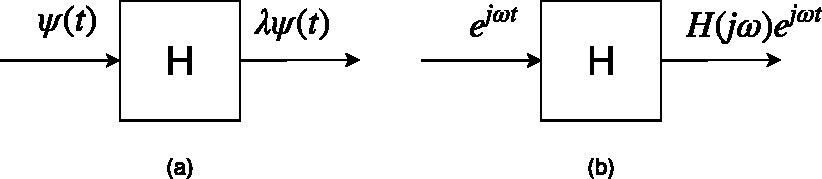
\includegraphics[width=0.8\linewidth]{Images/RevisaoDeLiteratura/PropriedadeDeAutofuncao.pdf}
	\caption{Ilustra��o da Propriedade de Autofun��o de Sistemas Lineares}
	\vspace{-3.5mm}
	\caption*{(a) Autofun��o geral $\psi (t)$ e  autovalor $\lambda$. }
	\vspace{-3.5mm}
	\caption*{(b) Autofun��o senoidal complexa $e^{i \omega t}$ e autovalor $H(j \omega)$.}
	\vspace{-3.5mm}
	\caption*{Fonte: Adaptado de \citeonline[p.~164]{Haykin}}
	\label{fig:PropriedadeDeAutofuncao}
\end{figure} 
\vspace{6mm}

A ideia principal aqui � utilizar a superposi��o ponderada de autofun��es para representar um �nico sinal peri�dico. Para esse efeito \citeonline[p.~164]{Haykin} expressa a entrada de um sistema LTI como uma soma de $N$ senoides complexas ponderadas, na forma: 

\begin{equation}
	x(t) = \sum_{k=1}^{N} a_k e^{j\omega_k t}
\end{equation}

Ou seja na forma de s�rie de Fourier.

Expressar a entrada de um sistema LTI a partir de uma soma ponderada de senoides complexas possui a inten��o de realizar uma aproxima��o coerente do sinal de entrada, utilizando uma composi��o de fun��es b�sicas j� bem conhecidas. Por exemplo considere o sinal de onda quadrada presente na Figura (\ref{fig:AproximacaoPorSomasDeSenoidesA.eps}), o qual deseja-se aproximar utilizando uma soma de senoides complexas. Tomando uma senoide de amplitude 1.286 e uma frequ�ncia de $50Hz$ � poss�vel realizar uma aproxima��o groseira, por�m em fase com este sinal.

\vspace{5mm}
\begin{figure}[H]
	\centering
	\captionsetup{width=0.7\textwidth, font=footnotesize, textfont=bf}	
	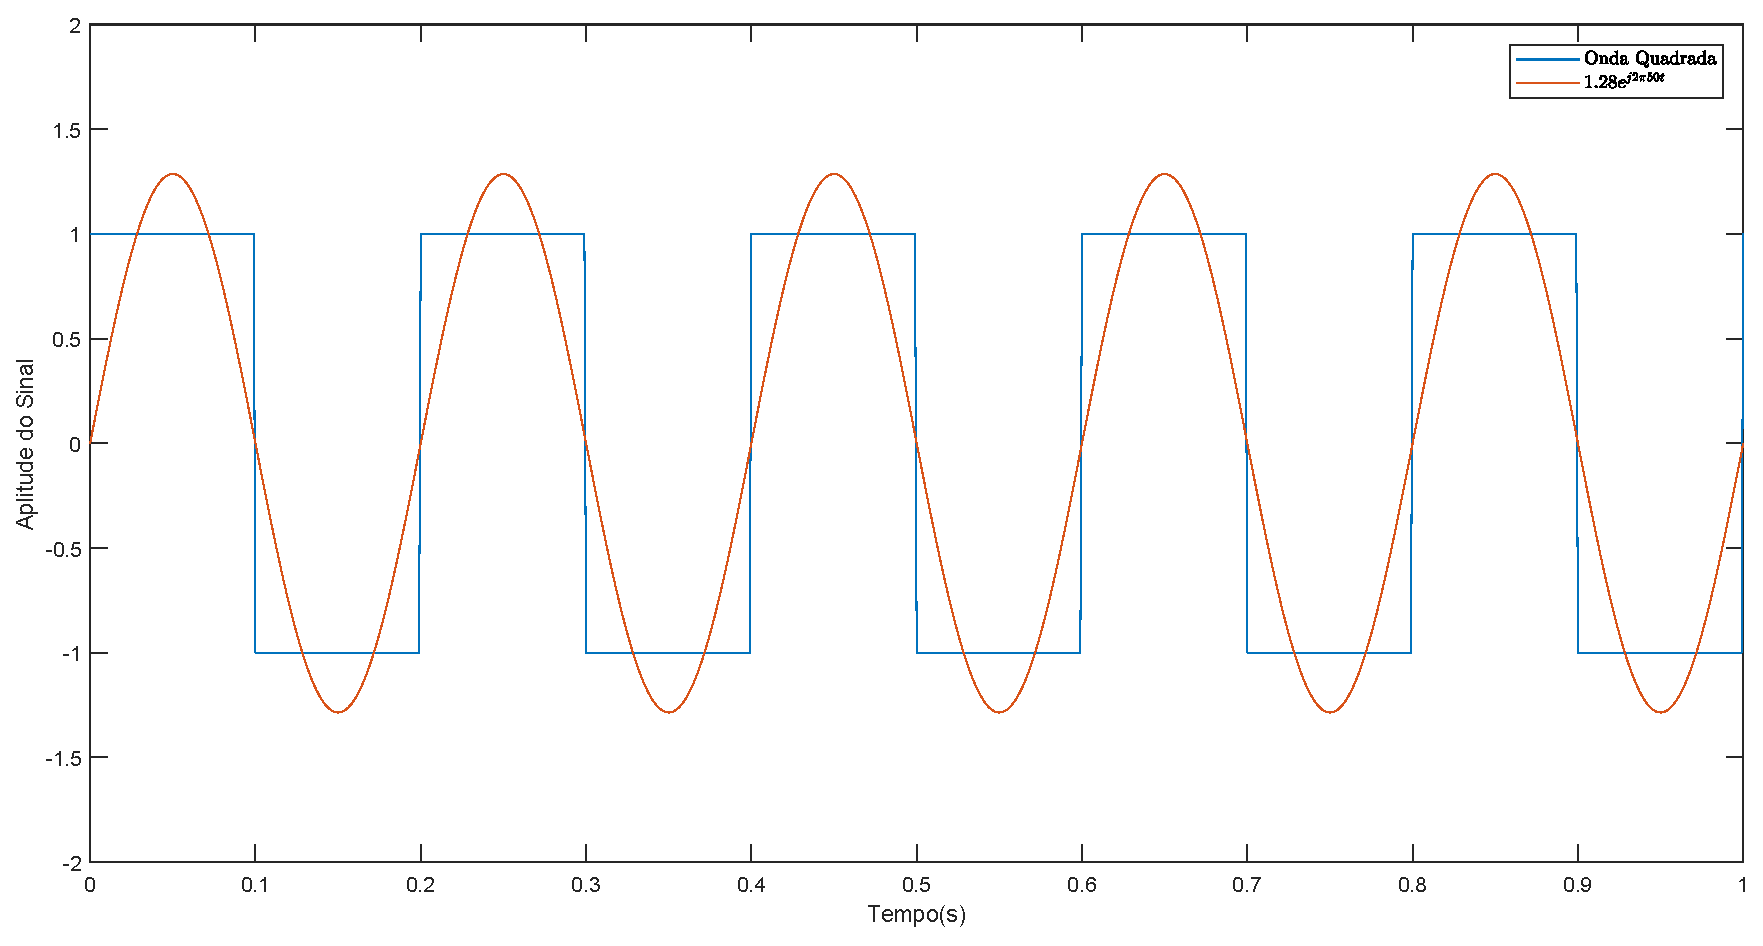
\includegraphics[width=0.7\linewidth]{Images/RevisaoDeLiteratura/AproximacaoPorSomasDeSenoidesA.eps}
	\caption{Aproxima��o do Sinal de Onda Quadrada por um Termo Senoidal}
	\vspace{-3.5mm}
	\caption*{Fonte: Autoria Pr�pria}
	\label{fig:AproximacaoPorSomasDeSenoidesA.eps}
\end{figure}
\vspace{5mm}

Para tornar melhorar a aproxima��o da representa��o em rela��o ao sinal de onda quadrada � poss�vel adicionado mais  termos senoidais ao somat�rio.  Como pode ser visto nas Figura (\ref{fig:AproximacaoPorSomasDeSenoidesB.eps}) e (\ref{fig:AproximacaoPorSomasDeSenoidesC.eps}) as aproxima��es ficam mais suaves adicionando mais 2 ou mais 5 termos respectivamente. Quanto maior o n�mero de termos senoidais complexas ponderados presentes no somat�rio da representa��o maior � a aproxima��o, sendo no limite perfeita.

\vspace{5mm}
\begin{figure}[H]
	\centering
	\captionsetup{width=0.7\textwidth, font=footnotesize, textfont=bf}	
	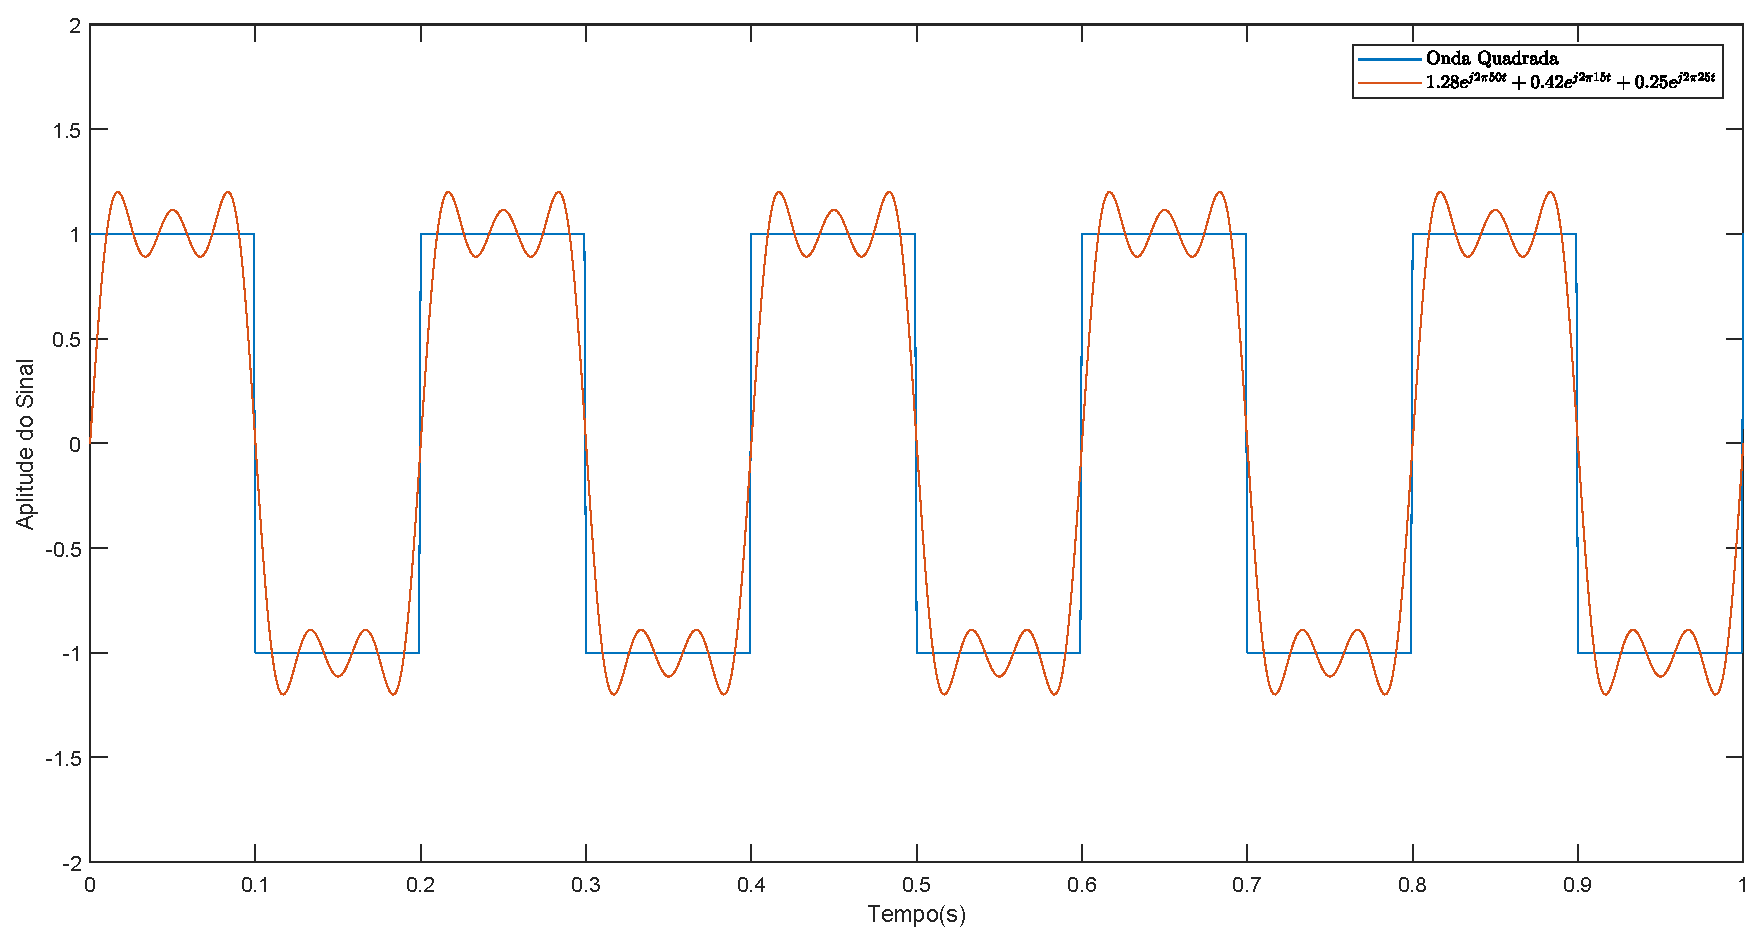
\includegraphics[width=0.7\linewidth]{Images/RevisaoDeLiteratura/AproximacaoPorSomasDeSenoidesB.eps}
	\caption{Aproxima��o do Sinal de Onda Quadrada por Soma de 3 Termos Senoidais}
	\vspace{-3.5mm}
	\caption*{Fonte: Autoria Pr�pria}
	\label{fig:AproximacaoPorSomasDeSenoidesB.eps}
\end{figure}
\vspace{5mm}
\begin{figure}[H]
	\centering
	\captionsetup{width=0.7\textwidth, font=footnotesize, textfont=bf}	
	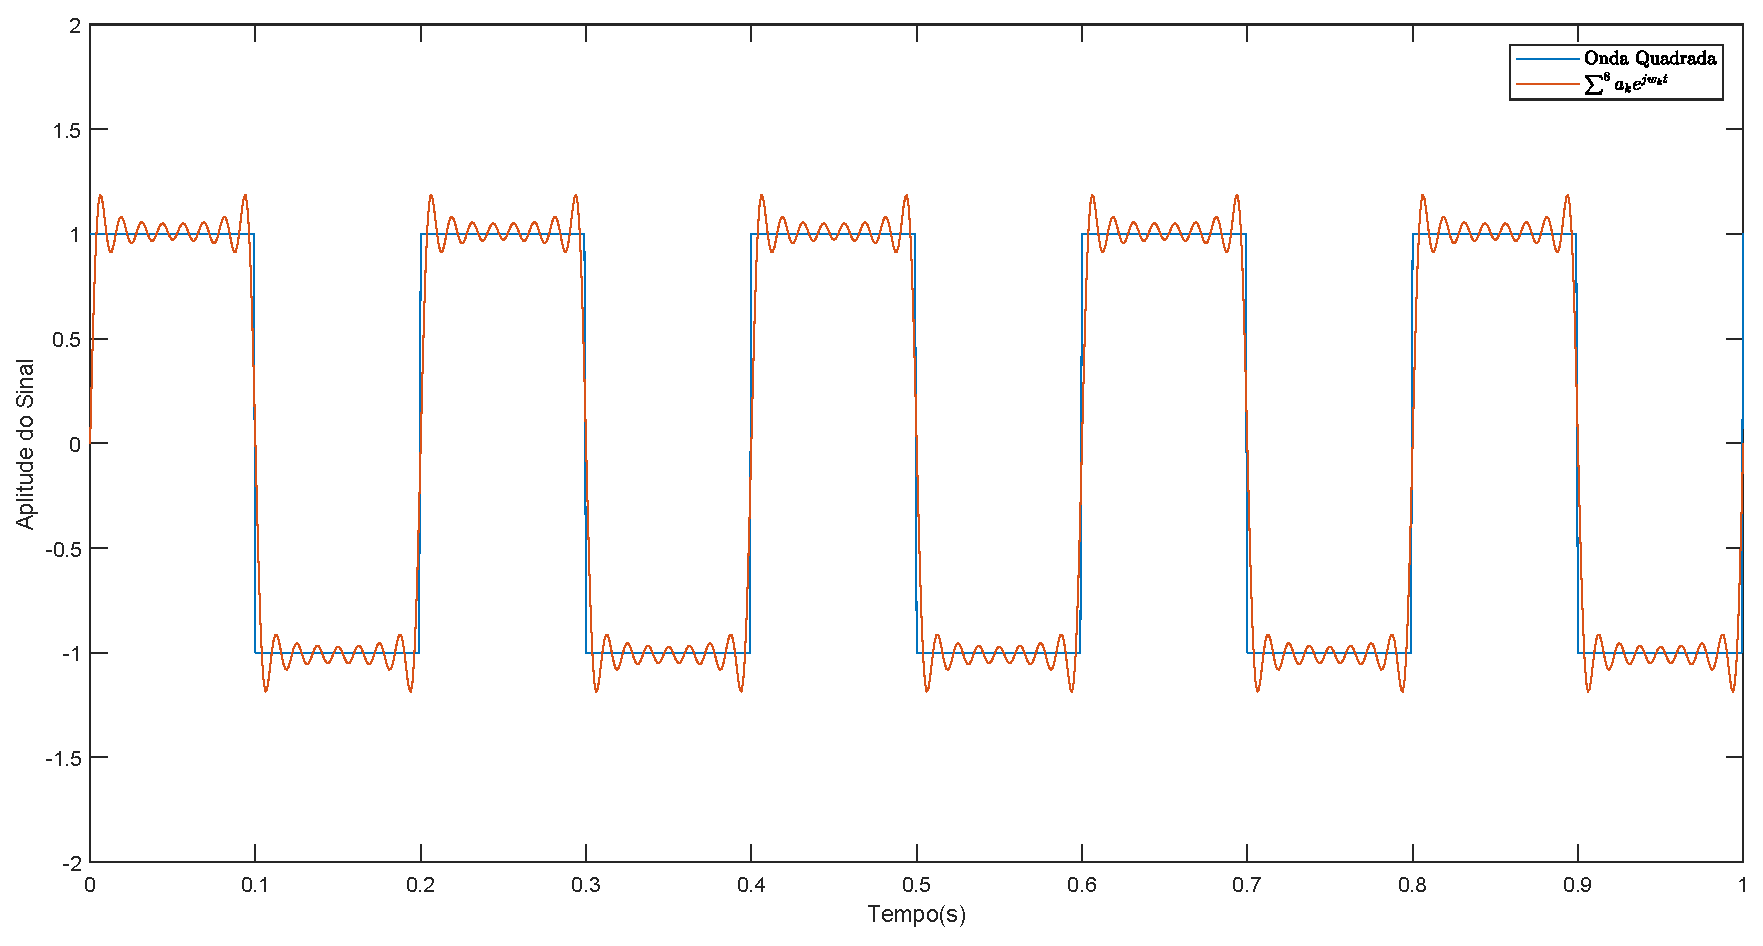
\includegraphics[width=0.7\linewidth]{Images/RevisaoDeLiteratura/AproximacaoPorSomasDeSenoidesC.eps}
	\caption{Aproxima��o do Sinal de Onda Quadrada por Soma de 8 Termos Senoidais}
	\vspace{-3.5mm}
	\caption*{Fonte: Autoria Pr�pria}
	\label{fig:AproximacaoPorSomasDeSenoidesC.eps}
\end{figure} 
\vspace{5mm}

Logo utilizando se $e^{j\omega_k t}$ for uma autofun��o e $H(j\omega_k)$ for o autovalor do sistema, aplicando-se a autorrela��o apresentada anteriormente, o sinal de sa�da do sistema e dado por:

\begin{equation}
	y(t) = \sum_{k=1}^{N} a_k H(j\omega_k)e^{j\omega_k t}
\end{equation}

A sa�da, portanto nada mais � do que a soma ponderada das senoides complexas da entrada, sendo os pesos $a_k$ ponderados pela resposta em frequ�ncia $H(j\omega_k)$. Por meio deste resultados � poss�vel transformar a opera��o de convolu��o em uma opera��o de multiplica��o dos termos $a_k~H(j\omega_k)$. Segundo \citeonline[p.~164]{Oppenheim} o fato da sa�da de um sistema LTI dada uma entrada representada como combina��o linear de senoides complexas, ser tamb�m uma combina��o linear dos mesmos sinais, foi uma descoberta de Euler, que motivou Fourier e os outros matem�ticos ap�s ele no estudo da extens�o de classes de sinais que poderiam ser representados nesta forma de somat�rios de exponenciais complexas ponderadas.

Al�m de tornar mais pr�tico o c�lculo da convolu��o de sinais, a representa��o em somais senoidais complexas ponderadas fornece uma interpreta��o alternativas para sinais e sistemas  \citeonline[p.~166]{Haykin}. Atrav�s da an�lise dos pesos  $a_k$ ponderados � poss�vel descrever um sinal em fun��o da frequ�ncia, ao inv�s do tempo. 

A representa��o de sinais por s�ries de Fourier pode ser aplicada para diferentes tipos de sinais, com diferentes caracter�sticas. H� quatro classes de representa��es de  Fourier, dividias de acordo com a sua periodicidade e sua continuidade, como poder ser visto na Tabela \ref{tab:PropriedadeTempoERepresentacaoFourier}. 

Para sinais peri�dicos a representa��o � feita como s�ries de Fourier, sendo que para sinais de tempo continuo � aplicado a S�rie de Fourier (FS - \textit{Fourier Series}), e para sinais de tempo discreto � usada as s�ries de Fourier de tempo discreto (DFS - \textit{Discrete Fourier Serie}). Quando os sinais n�o s�o peri�dicos a representa��o � denominada como transformada, para o caso do sinal ser cont�nuo a representa��o � feita pela transformada de Fourier (FT - \textit{Fourier Transform}), e no caso discreto � a transformada de Fourier de tempo discreto (DFT - \textit{Discrete Fourier Trasform}).

\vspace{6mm}
\begin{table}[h]
\centering
\captionsetup{width=0.9\linewidth}
\begin{tabular}{|c|c|c|}
	\hline
	Propriedade do Tempo                                                      & \cellcolor[HTML]{000000}{\color[HTML]{FFFFFF} Peri�dico} & \cellcolor[HTML]{000000}{\color[HTML]{FFFFFF} N�o Periodico} \\ \hline
	\cellcolor[HTML]{000000}{\color[HTML]{FFFFFF} }                           & S�rie de Fourier (FS)                                    & Transformada de                                              \\
	\multirow{-2}{*}{\cellcolor[HTML]{000000}{\color[HTML]{FFFFFF} Continuo}} & \multicolumn{1}{l|}{}                                    & Fourier (FT)                                                 \\ \hline
	\cellcolor[HTML]{000000}{\color[HTML]{FFFFFF} }                           & S�rie de Fourier de                                      & Transformada de Fourier de                                   \\
	\multirow{-2}{*}{\cellcolor[HTML]{000000}{\color[HTML]{FFFFFF} Discreto}} & \multicolumn{1}{l|}{Tempo Discreto (DFS)}                & \multicolumn{1}{l|}{Tempo DIscreto (DFT)}                    \\ \hline
\end{tabular}
\caption{Rela��o entre propriedade do tempo de um sinal e a representa��o de Fourier adequada}
\vspace{-3.5mm}
\caption*{Fonte: \citeonline[p.~166]{Oppenheim}}
\label{tab:PropriedadeTempoERepresentacaoFourier}
\end{table}
\vspace{6mm}

A representa��o de Fourier utilizada no desenvolvimento deste trabalho � a DFT, e portanto a mais importante a ser apresentada. As pr�ximas se��es deste trabalho passaram pela apresenta��o da FS depois pela DFS para em fim chegar na DFT. 

\subsection{S�rie de Fourier}

Segundo \citeonline[p.~530]{Lathi}  "Um sinal peri�dico $x(t)$ com per�odo $T_0$ pode ser descrito como a soma de senoides de frequ�ncia $f_0$ e todas as suas harm�nicas", conforme apresentado na Equa��o (\ref{eq:SerieFourierFundamental}). Esta � a chamada s�rie de Fourier para sinais peri�dicos, ou apenas s�rie de Fourier. Na express�o da Equa��o (\ref{eq:SerieFourierFundamental}) a s�rie de Fourier est� na forma trigonom�trica. Onde $\omega_0$ � a frequ�ncia fundamental de $x(t)$, e $a_0$, $a_n$ e $b_n$ s�o os coeficientes de amplitude das harm�nicas que comp�es $x(t)$, sendo $a_0$ a harm�nica zero (n�vel CC).


\begin{equation}
	x(t) ~=~ a_0 + \sum _{n=1} ^{\infty} a_n cos (n \omega_0 t) + b_n sen(n \omega_0 t)
	\label{eq:SerieFourierFundamental}
\end{equation}

Os coeficientes $a_0$, $a_n$ e $b_n$ da Equa��o (\ref{eq:SerieFourierFundamental} ) s�o determinados pelas seguintes equa��es: 

\begin{equation}
	a_0~=~\frac{1}{T_0} \int_{T_0} x(t) dt
	\label{eq:SerieFourierFundamentala0}
\end{equation}

\begin{equation}
	a_n~=~\frac{2}{T_0} \int_{T_0} x(t) cos(n \omega_0 t) dt
	\label{eq:SerieFourierFundamentalan}
\end{equation}

\begin{equation}
	b_n~=~\frac{2}{T_0} \int_{T_0} x(t) sen(n \omega_0 t) dt
	\label{eq:SerieFourierFundamentalbn}
\end{equation}

em que $T_0$ representa o per�odo relativo a frequ�ncia fundamental $f_0$.

� s�rie de Fourier, al�m da forma trigonom�trica, tamb�m pode ser apresentada na forma  exponencial, em termos de $e^{j \omega_0 t}$, como apresentado na se��o anterior. A forma exponencial, segundo \citeonline[p.~533]{Lathi}, � dada atrav�s da Equa��o (\ref{eq:SerieFourierExponencial}), em que o coeficiente $C_n$ e an�logo aos coeficientes $a_n$ e $b_n$ da serie trigonom�trica, sendo obtido por (\ref{eq:SerieFourierExponencialCn}) .

\begin{equation}
	x(t)~=~\sum^{\infty} _{- \infty} C_n e^{j n \omega_0 t}
	\label{eq:SerieFourierExponencial}
\end{equation}

\begin{equation}
	C_n~=~ \frac{1}{T_0} \int_{T_0} x(t) e^{j n \omega_0 t} dt
	\label{eq:SerieFourierExponencialCn}
\end{equation}

Tanto a forma trigonom�trica quanto a exponencial da s�rie de Fourier consideram $x(t)$como sendo uma fun��o qualquer, real ou complexa. Por�m na maioria das aplica��es $x(t)$ � real, como � o caso dos sinais neste trabalho. Segundo segundo \citeonline[p.~533]{Lathi}, se o sinal de entrada do sistema LTI $x(t)$ � real, isso significa que $a_n$ e $b_n$ tamb�m s�o reais para todos os valores de $n$, sendo portanto a s�rie  de Fourier representada na forma compacta:

\begin{equation}
	x(t) = D_0 + \sum_{n=1}^{\infty} D_n cos(n \omega_0 t + \theta_n)
	\label{eq:FourierCompact}
\end{equation}

Sendo:

\begin{equation}
	D_0 = a_0
\end{equation}

\begin{equation}
	D_n = \sqrt{a_n^2 + b_n^2}
\end{equation}

\begin{equation}
	\theta_n = tan^{-1} \frac{-b_n}{a_n}
\end{equation}

Utilizar $cos $

\subsection{Espectro de Fourier}

Por meio da s�rie de Fourier na forma compacta, apresentada na Equa��o \ref{eq:FourierCompact}, conclui-se que um sinal real peri�dico $x(t)$ pode ser descrito como uma soma de senoides de frequ�ncias $n \omega_0$ e amplitudes $D_n$ e fases $\theta_n$. Segundo \citeonline[p.~533]{Lathi}, o espectro exponencial de Fourier � tra�ado a partir de $D_n$ e $\theta_n$ em fun��o das frequ�ncias $n \omega_0$. Logo s�o ta�ados dois gr�ficos para o espectro exponencial de Fourier, um que relaciona $C_n$ com $n \omega_0$, chamado espectro de magnitude. E outro que relaciona $\theta_n$ com $n \omega_0$, chamado de espectro de fase.

Tomando como exemplo um sinal $x(t)~=~sin(2 \pi 15t) + sin(2\pi40t)$, expresso em um per�odo igual a 1 segundo, como mostrado na Figura \ref{fig:EspectroDeFourier}. Para este sinal e expresso o espectro de Fourier na mesma Figura (\ref{fig:EspectroDeFourier}), com o espectro de magnitude e fase. 

\vspace{5mm}
\begin{figure}[H]
	\centering
	\captionsetup{width=0.9\textwidth, font=footnotesize, textfont=bf}	
	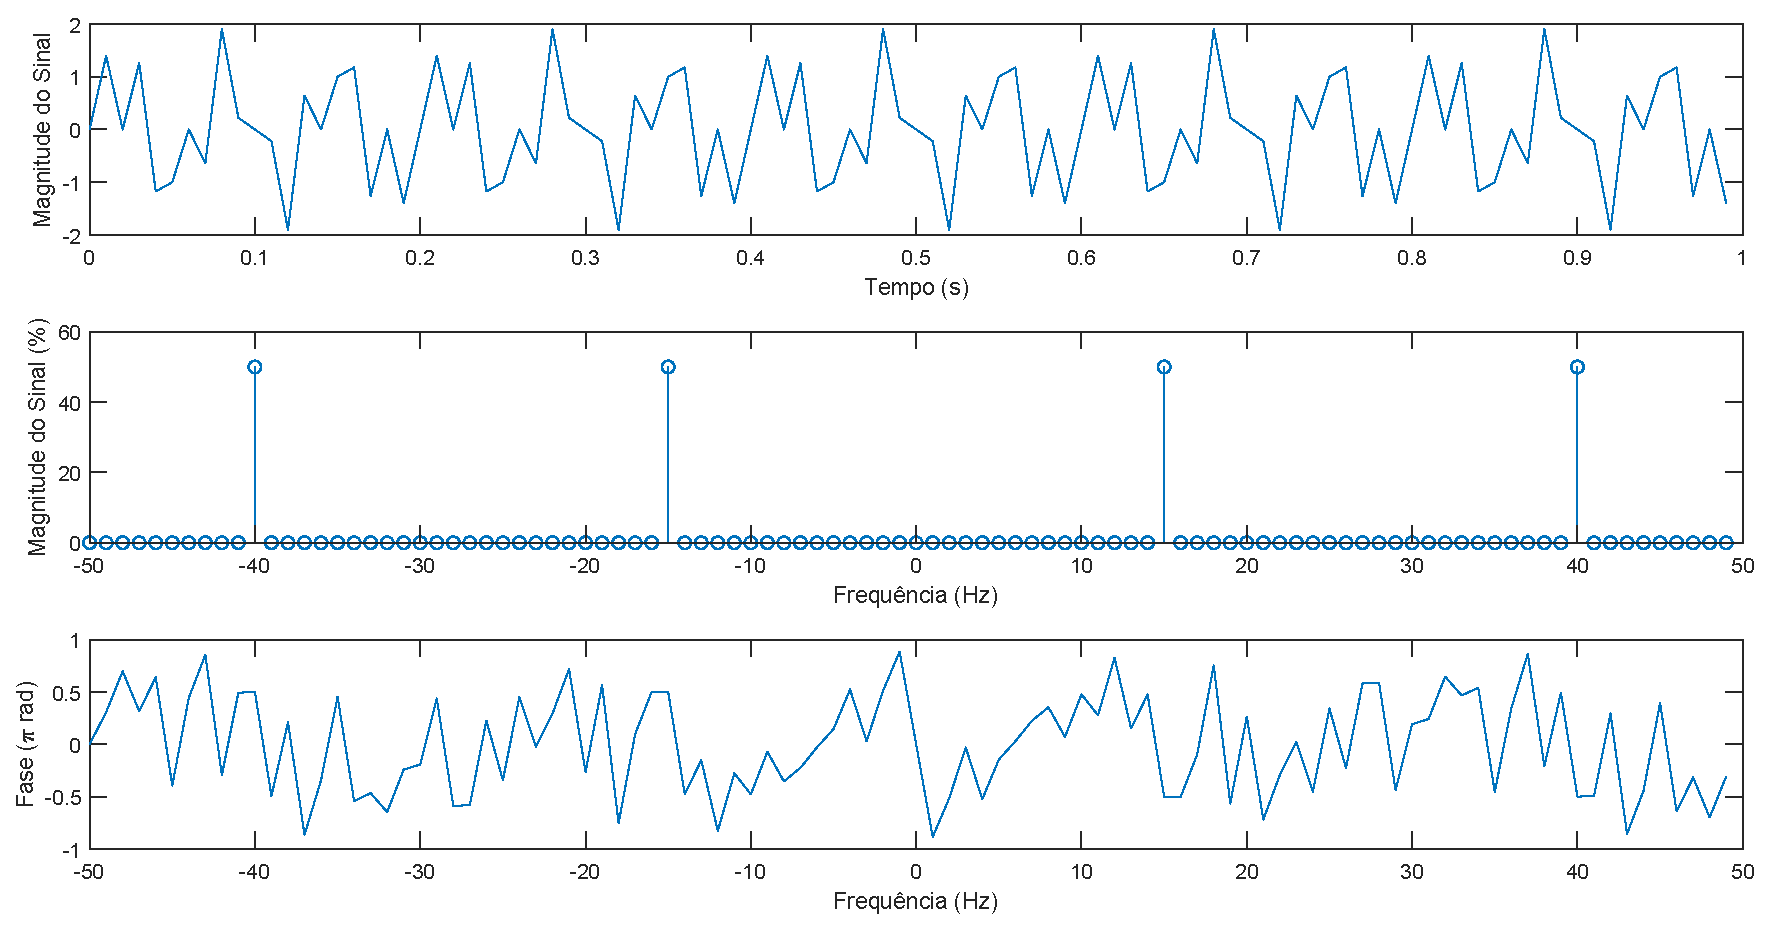
\includegraphics[width=0.9\linewidth]{Images/RevisaoDeLiteratura/EspectroDeFourier.eps}
	\caption{Aproxima��o do Sinal de Onda Quadrada por Soma de 8 Termos Senoidais}
	\vspace{-3.5mm}
	\caption*{Fonte: Autoria Pr�pria}
	\label{fig:EspectroDeFourier}
\end{figure} 
\vspace{5mm}

Nota-se que o espectro da Figura  (\ref{fig:EspectroDeFourier}) aparecem frequ�ncias negativas, as quais dividem a magnitude com suas frequ�ncias sim�tricas. Isso ocorre devido a simetria do angulo $n \omega_0 t$ possui no calculo dos coeficientes da s�rie de Fourier. Para resolver este problema basta considerar apenas a parte positiva do espectro e multiplicar por 2 a magnitude das frequ�ncias no espectro de magnitude. 

Para \citeonline[p.~533]{Lathi} os dois gr�ficos de magnitude e fase juntos formam o espectro de frequ�ncia, o qual revela os conte�dos de frequ�ncia do sinal $x(t)$, com suas amplitudes e fase. Conhecendo-se este espectro n�o s� � poss�vel analisar o sinal $x(t)$ dentro do dom�nio da frequ�ncia, como tamb�m reconstru�-lo de forma f�cil .

	
\section{S�rie de Fourier em Tempo Discreto}
	Ate aqui foi apresentada a forma continua da s�rie de Fourier, por�m para ser �til em uma aplica��o computacional � necess�rio encontrar sua forma discreta, ou DFT \textit{(Discrete Fourier Transform)}. Segundo HAYKIN e Veen (2001, p. 314) a DFT �
a �nica representa��o de Fourier que pode ser calculada por um computador, sendo amplamente usada para manipular sinais.

O primeiro passo para se obter uma DFT e considerar o teorema da Amostragem. Tal teorema afirma que um sinal real $x(t)$, cujo o espectro e limitado em $\phi~Hz$, pode ser reconstru�do a partir de suas amostras tomadas uniformemente a uma taxa $f_s \textgreater 2 \phi$ \cite[p.~679]{Lathi}. Em seguida, a amostragem de $x(t)$, feita a
uma frequ�ncia $f_s$, pode ser obtida pela multiplica��o de $x(t)$ por um trem de impulsos $\delta (t)$. Sendo tais impulsos unit�rios e peri�dicos, repetidos a cada  $T~=~1/f_s$ segundos, por um numero total de amostras $N_0$, a amostragem pode ser definida por:

\begin{equation}
	\overline{x}(t)~=~x(t) \delta_{T}(t)~=~\sum^{N_0 -1} _{n=0} x(nT) \delta(t-nT)
	\label{eq:FourierAmostragem}
\end{equation}

Por conveni�ncia, deseja-se obter um espectro do sinal amostrado $x(t)$ em fun��o de $\omega$ ou expresso em termos de frequ�ncia. Para tal, segundo \citeonline[p.~681]{Lathi}, o trem de impulsos $\delta(t)$ e um sinal peri�dico que pode ser descrito pela s�rie trigonom�trica de Fourier da seguinte forma:

\begin{equation}
	\delta_T (t)~=~\frac{1}{T} [1+ 2cos(\omega_s t) + 2cos(2\omega_s t) + 2cos(3\omega_s t) + \dotsc]
	\label{eq:TremDeImpulsos}
\end{equation}

Logo, multiplicando $x(t)$ por $\delta_{T} (t)$, obtem-se:

\begin{equation}
	\overline{x}(t)~=~x(t) \delta_{T}(t)~=~\frac{1}{T} [x(t) + 2x(t)cos(\omega_s t) + 2x(t)cos(2 \omega_s t) + 2x(t)cos(3 \omega_s t) + \dotsc]
	\label{eq:FourierAmostragemTremDeImpulsos}
\end{equation} ?

Segundo \citeonline[p.~125]{Oppenheim}, a transformada de Fourier do primeiro termo $x(t)$, em (\ref{eq:FourierAmostragemTremDeImpulsos}), � $X(\omega)$. J� a transformada de Fourier do segundo termo 2x(t)cos(!st) � $X(\omega ? \omega_s)~+~X(\omega + \omega_s)$, e do terceiro termo $2x(t)cos(2 \omega_s t)$ �
$X(\omega ? 2 \omega_s) + X(\omega + 2 \omega_s)$. E assim, semelhantemente a transformada de Fourier dos demais termos da serie que descreve (\ref{eq:FourierAmostragemTremDeImpulsos}), representam o espectro $X(\omega)$ deslocado em $n\omega_s$ e $?n\omega_s$. Assim,

\begin{equation}
	\overline{X}( \omega )~=~ \frac{1}{T} \sum_{\infty}^{-\infty} X(\omega - n \omega_s)
	\label{eq:FourierAmostragemDeslocada}
\end{equation}

Desde que a frequ�ncia de amostragem $f_s$ garanta o crit�rio do teorema da Amostragem, o sinal $\overline{X}$ ser� constitu�do de repeti��es n�o sobrepostas de $x(\omega_0)$, a um intervalo de tempo $T = 1/f_s$. Logo tanto $\overline{X}(\omega)$, quanto $\overline{x}(t)$ s�o peri�dicas e equivalentes, por�m com representa��es distintas do especto amostrado. Sendo assim, atrav�s da propriedade de deslocamento no tempo da transformada de Fourier (\ref{eq:Impulso}) e da e (\ref{eq:FourierAmostragem}), obt�m-se (\ref{eq:FourierAmostragemExponencial}) \citeonline[p.~125]{Oppenheim}:

\begin{equation}
	\delta(t - nT) \longleftrightarrow e^{-jn \omega T }
	\label{eq:Impulso}
\end{equation}

\begin{equation}
	\overline{x}(t)~=~\sum_{n=0}^{N_0 - 1} x(nT)e^{-j n \omega T}
	\label{eq:FourierAmostragemExponencial}
\end{equation}

Segundo \citeonline[p.~705]{Lathi}, a transformada de $\overline{x}(t)$ pode ser aproximada, considerando um certo \textit{aliasing} negligenci�vel, para $X(\omega)/T$. Portanto:

\begin{equation}	
	X(\omega)~=~T \sum_{n=0}^{N_0 - 1} x(nT) e^{j n \omega T} ~~ |\omega| \leq \frac{\omega_s}{2}
	\label{eq:DefinicaoDFT}	
\end{equation}

Analisando a propriedade peri�dica de $x(t)$ e $X(\omega)$, e considerando $x(nT)$ e $X(r\omega_0)$ a n-�sima e r-�sina amostra de $x(t)$ e $X(\omega)$, respectivamente, s�o definidas as seguintes vari�veis:

\begin{equation}
	x_n~=~Tx(nT)
	\label{eq:DefinicaoDFTA}
\end{equation}

\begin{equation}
	x_n~=~\frac{T_0}{N_0}x(nT)
	\label{eq:DefinicaoDFTB}
\end{equation}

\begin{equation}
	X_r ~=~ X ( \omega )
	\label{eq:DefinicaoDFTC}
\end{equation}

\begin{equation}
	\omega~=~r \omega_0
	\label{eq:DefinicaoDFTD}
\end{equation}

\begin{equation}
	X_r~=~X(r \omega_0)
	\label{eq:DefinicaoDFTE}
\end{equation}

\begin{equation}
	\omega_0~=~2 \pi f_0 ~=~\frac{2 \pi}{T_0}
	\label{eq:DefinicaoDFTF}
\end{equation}

Assim, substituindo (\ref{eq:DefinicaoDFTE}) e (\ref{eq:DefinicaoDFTB}) em (\ref{eq:DefinicaoDFT}), e fazendo $\omega_0 T = \Omega_0 = 2 pi /N_0$, se
obt�m a seguinte express�o para a transformada discreta de Fourier \cite[p.~125]{Oppenheim}:

\begin{equation}
	X_r~=~\sum_{n=0}^{N_0 - 1} x_n e^{j \omega_0 n r}
	\label{eq:DefinicaoDFTG}
\end{equation}

Onde:

\begin{equation}
	\Omega_0~=~\frac{2 \pi}{N_0}
	\label{eq:DefinicaoOmega}
\end{equation}

Para compactar a express�o de (\ref{eq:DefinicaoDFTG}) se faz a substitui��o da express�o exponencial pela vari�vel  $W$, de modo que $W_{N_0} = e^{?2 \pi /N_0} = e^{-j \Omega_0}$. Logo a express�o para DFT � dada por (\ref{eq:DFT}) \cite[p.~344]{meyer}:

\begin{equation}
	X_r~=~\sum_{n=0}^{N_0 - 1} x_n e^{j \omega_0 n r}
	\label{eq:DFT}
\end{equation}

Onde:

\begin{equation}
	0 \leq k  \leq N_0 - 1
	\label{eq:N0}
\end{equation}


	
\section{Transformada R�pida de Fourier}
	
Para se calcular uma DFT de $N_0$ valores usando apenas (\ref{eq:DFT}), � necess�rio realizar um total de $N^2_0$ multiplica��es e  $N_0(N_0 - 1)$ somas, utilizando n�meros complexos. Deste modo, quando $N_0$ assume um valor elevado, muitos recursos computacionais s�o necess�rios, at� chegar ao ponto de que esse algoritmo se torna impratic�vel.

A redu��o do numero de opera��es matem�ticas necess�rias para calcular a DFT � poss�vel a partir do algoritmo criado por J.W. Cooley e John Tukey, conhecido como Transformada R�pida de Fourier ou FFT \textit{(Fast Fourier Transform)} \citeonline[p.~719]{Lathi}. Para reduzir o numero de c�lculos, a FFT se utiliza da propriedade linear da transformada de Fourier. Segundo \citeonline[p.~119]{Oppenheim}, a transformada de Fourier de um sinal pode ser dada pela combina��o linear da transformada de Fourier de segmentos menores do mesmo sinal. Logo, � poss�vel aplicar a DFT o paradigma da Divis�o e Conquista, o qual � um recurso muito utilizado em algoritmos de ordena��o. 

Segundo \citeonline[p.~21]{Cormen}, um algoritmo de Divis�o e Conquista realiza o desmembramento de um problema em v�rios subproblemas que s�o id�nticos ao original, por�m menores em sua faixa de a��o, o que os torna mais simples de resolver. Em seguida, resolvem-se os subproblemas recursivamente e combinam-se essas solu��es de modo a obter a solu��o para o problema original.

De modo muito semelhante, o algoritmo da FFT prev� uma divis�o recursiva  da DFT em dois blocos: bloco par e o bloco �mpar, como mostrado abaixo\cite[p.~35]{Chu}: 

\begin{equation}
	X_r~=~\underbrace{\sum^{\frac{N_0}{2} - 1}_{n=0} x_{2n} W^{2nr}_{N_0}}_{Parcela~Par} ~ + ~\underbrace{\sum^{\frac{N_0}{2} - 1}_{n=0} x_{2n+1} W^{(2n+1)r}_{N_0}}_{Parcela~\acute{I}mpar}.
	\label{eq:DenicaoFFT}  
\end{equation}

Nesta mesma equa��o os limites dos somat�rios de ambas as parcelas �mpar e par foram redefinidas para englobar apenas metade dos $N_0$ pontos, bem como os expoentes de $W$ foram ajustados.

Utilizando algumas das propriedades geom�tricas de $W$, j� que este representa um numero complexo, pode-se realizar simplifica��es importantes em \ref{eq:DenicaoFFTA}. Primeiro, nota-se que $W_{N_0 / 2}~=~W_{N_0} ^{2}$, logo:

\begin{equation}
	X_r~=~\underbrace{\sum^{\frac{N_0}{2} - 1}_{n=0} x_{2n} W^{2nr}_{N_0}}_{G_r} ~ + ~\underbrace{\sum^{\frac{N_0}{2} - 1}_{n=0} x_{2n+1} W^{(2n+1)r}_{N_0}}_{H_r}.
	\label{eq:DenicaoFFTA}  
\end{equation}

Como $G_r$ e $H_r$ s�o DFTs com $N_0 / 2$ pontos cada, ent�o ambos possuem um per�odo de $N_0 / 2$. Com base na propriedade peri�dica destas DFTs, pode-se utilizar as simplifica��es (\ref{eq:Gr}) e (\ref{eq:Hr}) para reduzir o n�mero de c�lculos na DFT \cite[p. 721]{Lathi}.

\begin{equation}
	G_{r+ \frac{N_0}{2}}~=~G_{r},
	\label{eq:Gr}
\end{equation}

\begin{equation}
	H_{r+ \frac{N_0}{2}}~=~H_{r},
	\label{eq:Hr}
\end{equation}

\begin{equation}
	W_{N_0} ^{r+\frac{N_0}{2}}~=~W_{N_0} ^{\frac{N_0}{2}}~=~e^{-j \pi} W_{N_0}~=~-W^{r}_{N_0}.
	\label{eq:WN}
\end{equation}

Al�m disso, a express�o em (\ref{eq:WN}) pode ser assumida para se reduzir o n�mero de c�lculos da FFT. Portanto, usando (\ref{eq:Xr}) e (\ref{eq:Xr1}) se obt�m, respectivamente, os primeiros $N_0/2$ pontos e os �ltimos $N_0/2$ pontos da FFT:

\begin{equation}
	W_{N_0} ^{r+\frac{N_0}{2}}~=~W_{N_0} ^{\frac{N_0}{2}}~=~e^{-j \pi} W_{N_0}~=~-W^{r}_{N_0},
	\label{eq:Xr}
\end{equation}

\begin{equation}
	W_{N_0} ^{r+\frac{N_0}{2}}~=~W_{N_0} ^{\frac{N_0}{2}}~=~e^{-j \pi} W_{N_0}~=~-W^{r}_{N_0},
	\label{eq:Xr1}
\end{equation}

Portanto, uma DFT pode ser calculada combinando duas DFTs de $N_0/2$, tal
como mostrado em (\ref{eq:Xr}) e (\ref{eq:Xr1}). � comum na literatura representar este processo de c�lculo de DFT feito pelo algoritmo da FFT pelo diagrama da Figura (\ref{fig:Butterfly}). Este diagrama � conhecido como \textit{Butterfly} de Fluxo do Sinal \cite[p.~36]{Chu}.

\vspace{4mm}
\begin{figure}[H]
	\centering
	\captionsetup{width=0.5\textwidth, font=footnotesize, textfont=bf}	
	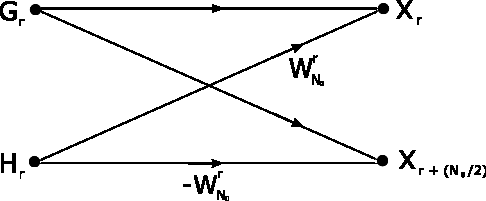
\includegraphics[width=0.5\linewidth]{Images/RevisaoDeLiteratura/Butterfly.pdf}
	\caption{Butterfly do Fluxo do Sinal}
	\vspace{-3.5mm}
	\caption*{Fonte: \citeonline[p.~721]{Lathi}}
	\label{fig:Butterfly}
\end{figure}
\vspace{4mm}

Aliando o conceito de divis�o em conquista ao m�todo de c�lculo da DFT, usando o diagrama \textit{Butterfly}, a representa��o do algoritmo da FFT pode ser facilmente representado pelo diagrama da Figura (\ref{fig:FFT8P}) \cite[p.~722]{Lathi}. Nesta figura, a FFT  � feita para apenas 8 amostras de sinal $X$.

\vspace{4mm}
\begin{figure}[H]
	\centering
	\captionsetup{width=1\textwidth, font=footnotesize, textfont=bf}	
	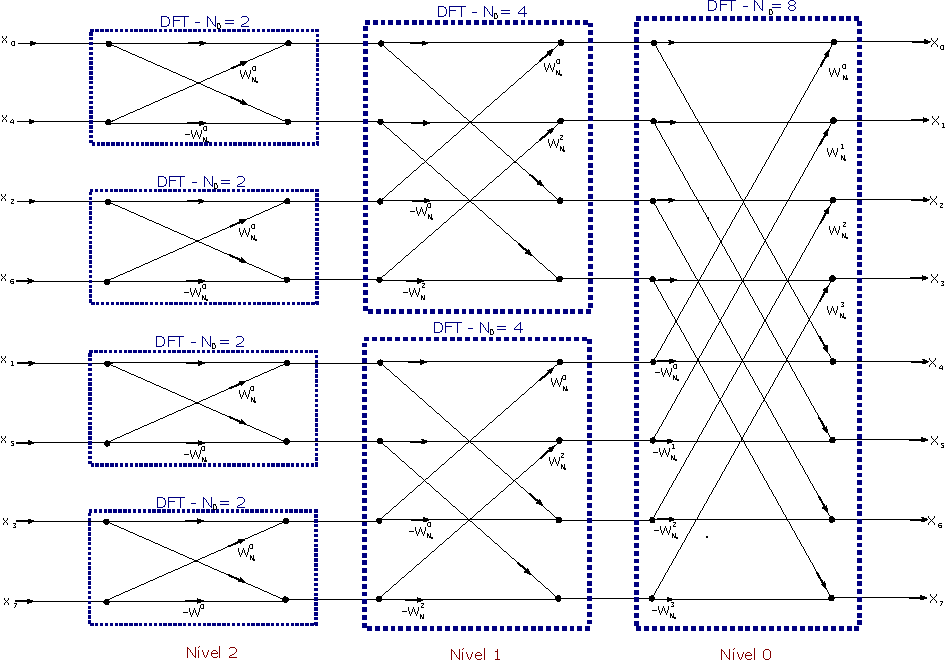
\includegraphics[width=1\linewidth]{Images/RevisaoDeLiteratura/FFT8P.pdf}
	\caption{FFT de 8 Pontos}
	\vspace{-3.5mm}
	\caption*{Fonte: \citeonline[p.~722]{Lathi}}
	\label{fig:FFT8P}
\end{figure}
\vspace{4mm}

Ap�s se dividir uma DFT de tamanho $N_0$ em duas DTFs de tamanho $N_0/2$,
e subdividindo cada uma das DFTs de tamanho $N_0/2$ em duas $N_0/4$ \cite[p.~721]{Lathi}. E assim o procedimento continua ate que se atinja um n�vel em que as DFTs tenham tamanho $N_0 / 2^n = 2$, ou seja, quando se atinge DFTs que possuam um custo de c�lculo m�nimo.

Um fato importante sobre o algoritmo da FFT � que o valor $N_0$ pode ser escolhido segundo a rela��o $N_0~=~r_n$, onde $n$ � o numero de n�veis necess�rios para calcular a FFT, e $r$ � o m�nimo tamanho DFT. Os algoritmos de FFT mais usados possuem a base $r$ igual a 2 ou a 4. Consequentemente, estes algoritmos s�o
conhecidos como Radix-2 e Radix-4, respectivamente \cite[p.~365]{Meyer}. Neste trabalho o foco ser� o algoritmo com a base $r$ igual a 2, ou seja, o Radix-2.

Na Figura (\ref{fig:FFT8P}) as DFTs est�o agrupadas por n�veis, onde cada n�vel abrange as DFTs de mesmo tamanho $N_0/n$, e no �ltimo n�vel a esquerda h� quatro DFTs de tamanho 2. O n�mero de n�veis necess�rios em uma FFT de $N_0$ pontos � $log_2 N_0$. Os valores de $X$, na Figura (\ref{fig:FFT8P})  � direita est�o ordenados de forma crescente, por�m os valores de $x$ � esquerda est�o ordenados de forma diferente. Est� ordena��o � conhecida como \textit{Bit-Reverse} \cite[p.~51]{Chu}.

Segundo \citeonline[p.~51]{Chu}, quando se divide o processo de c�lculo de uma DFT em duas, sendo uma respons�vel pelos valores pares e a outra pelo valores �mpares, conforme as conex�es entres o n�veis v�o ocorrendo, h� permuta��es entre os sinais. O processo de \textit{Bit-Reverse} prev� estas permuta��es, sendo poss�vel saber qual a ordem adequada dos sinais na entrada da FFT. Para aplicar o conceito de \textit{Bit-Reverse}, basta considerar um elemento $x_k$ de ordem $n$ e escrev�-lo na base binaria com $log_2 N_0$ bits. Em seguida, para determinar onde $x_k$ ser� ocupado, basta converter novamente para base decimal o n�mero bin�rio obtido, lendo esse na ordem inversa dos bits.

Na FFT da Figura (\ref{fig:FFT8P}) a subdivis�o das DFTs � deita a partir da sa�da, sinal em frequ�ncia, com DFT de 8 pontos, at� a entrada, sinal no tempo, com as DFTs de 2 pontos com custo m�nimo. Essa subdivis�o � conhecida como decima��o, e no caso da Figura (\ref{fig:FFT8P}), ela � feita a partir do sinal no tempo, logo essa estrutura � conhecida como Decima��o no Tempo. Por�m, existe uma outra forma, a decima��o na frequ�ncia. A partir de uma altera��o em (\ref{eq:DenicaoFFTA}), � poss�vel alterar a ordem da decima��o, partindo do sinal de entrada no tempo, at� a sa�da em frequ�ncia, como pode ser visto na Figura(\ref{fig:FFT8PDIF}) \cite[p.~37]{Chu}.

\vspace{4mm}
\begin{figure}[H]
	\centering
	\captionsetup{width=1\textwidth, font=footnotesize, textfont=bf}	
	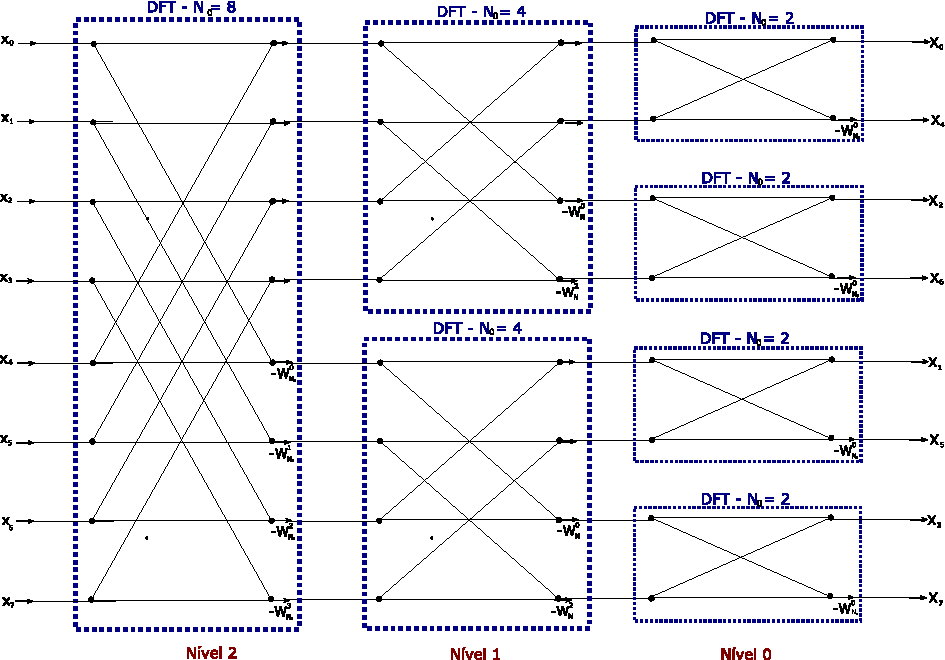
\includegraphics[width=1\linewidth]{Images/RevisaoDeLiteratura/FFT8PDIF.pdf}
	\caption{FFT DIF de 8 Pontos}
	\vspace{-3.5mm}
	\caption*{Fonte: Adaptado de \citeonline[p.~44]{Chu}}
	\label{fig:FFT8PDIF}
\end{figure}
\vspace{4mm}

Na decima��o em frequ�ncia, a ordem de entrada dos sinais na FFT ficar ordenados de forma crescente, por�m a sa�da passa a estar ordenado no esquema \textit{Bit-Reverse}. Este esquema de decima��o � preferencialmente escolhido por dispensar a reordena��o dos dados de entrada.

Ao final de todo o processo de simplifica��o do c�lculo da DFT, o algoritmo da FFT necessita apenas realizar $(N_0/2)~log_2~N_0$ multiplica��es e $N_0~log_2~N_0$ somas
complexas \cite[p.~720]{Lathi}. Desta forma, reduz-se assim a complexabilidade do
algoritmo, tornando a DFT pratic�vel at� para valores elevados de $N_0$.

	
\section{FPGA}
	%Como afirma \citeonline[Pref�cio]{Meyer}, muitos algoritmos de processamento de sinais, como FFT \textit{(Fast Fourier Transform)} e os filtros FIR ou IIR, implementados anteriormente em PDSPs ou em Circuitos Integrados de Aplica��o Especifica ou ASIC \textit{(Application Specific Integrated Circuits)}, agora est�o sendo implementados em FPGAs.

\citeonline{moore}[p.~4] define a FPGA como um dispositivo semicondutor capaz de ser totalmente redefinido ap�s sua fabrica��o, permitindo ao desenvolvedor reconfigurar produtos e fun��es j� implementadas, adaptando o \textit{hardware} a novas fun��es. De forma pr�tica, a FPGA permite uma flexibilidade em um projeto, podendo mudar a forma como ele � implementado, sem a necessidade de se construir um \textit{hardware} novo.

\vspace{5mm}
